\documentclass[letterpaper,10pt]{article}
\usepackage[top=2cm, bottom=1.5cm, left=1cm, right=1cm]{geometry}
\usepackage{amsmath, amssymb, amsthm,graphicx, enumitem}
\usepackage{fancyhdr}
\pagestyle{fancy}

\lhead{\today}
\chead{Quality Engineering Assignment 7}
\rhead{Justin Hood}

\newcommand{\Z}{\mathbb{Z}}
\newcommand{\Q}{\mathbb{Q}}
\newcommand{\R}{\mathbb{R}}
\newcommand{\C}{\mathbb{C}}
\newtheorem{lem}{Lemma}

\begin{document}
\begin{enumerate}
\item Paint Non-conformities\\
We consider the data below,
\begin{center}
\begin{tabular}{|l|r|r|r|}
\hline
 & Frequency & Cost/Unit & Total Cost\\\hline
Blister & 212 & 0.5 & 106 \\\hline
Light Spray & 582 & 0.1 & 58.2 \\\hline
Drips & 227 & 0.4 & 90.8 \\\hline
Overspray & 109 & 0.25 & 27.25\\\hline
Splatter & 141 & 0.35 & 49.35\\\hline
Bad Paint & 126 & 3 & 378\\\hline
Runs & 434 & 1.5 & 651\\\hline
\end{tabular}
\end{center}
We construct the Pareto Analysis by Total Cost, the result follows,
\begin{center}
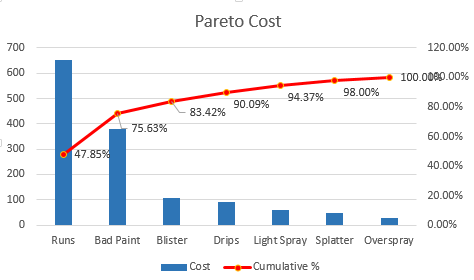
\includegraphics[scale=1]{1costpareto.png}
\end{center}
We see from the cost analysis that the Runs in the paint contribute the most to the overall cost of repairs; nearly half of the overall cost. Over $90\%$ of the overall cost is attributed to only four types of issue. From a business stand point, we would want to fix the runs in the paint, as well as improve the overall supply of paint to cut cost first.
\item We consider the check sheet for the aircraft landing gears produced by company PT. Using Excel, we obtain the following Pareto Chart,
\begin{center}
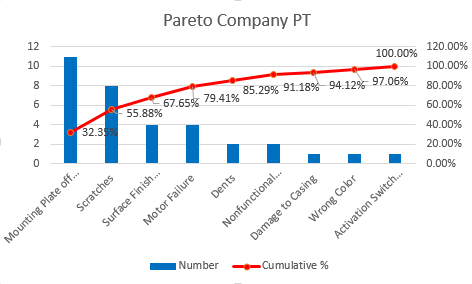
\includegraphics[scale=1]{2checkpareto.png}
\end{center}
Based on this analysis, we see that the Mounting Plate contributes the most to the overall repair percentage, but the category of Finish Flaws seem to have a majority on the left end of the Pareto Chart, as such, we will probably want to focus on improving the finishing process to reduce the overall repair quantity.
\item Using the same data from before, but now with the cost per repair added we construct the Pareto chart by cost for comparison.
\begin{center}
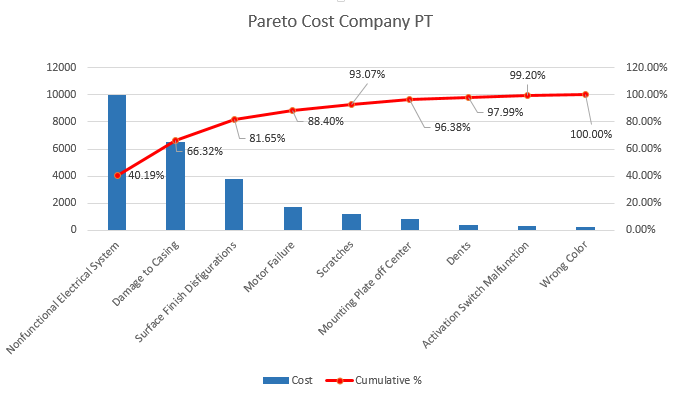
\includegraphics[scale=1]{3costpareto.png}
\end{center}
From this analysis, we see that nonfunctioning electrical systems are the highest cost to the company by ratio, contributing $40\%$ of the overall repair cost. In addition, by looking at the relative contributions of each category, (Finish and Operational) We see that the Operational defects contribute more to the overall repair cost, but by very little more than the Finish Defects.
\item See Attached Word Document ``Problem 4 Flow Chart"
\item See Attached Word Document ``Problem 5 Diagram"
\item Using the data provided, we construct a histogram.
\begin{center}
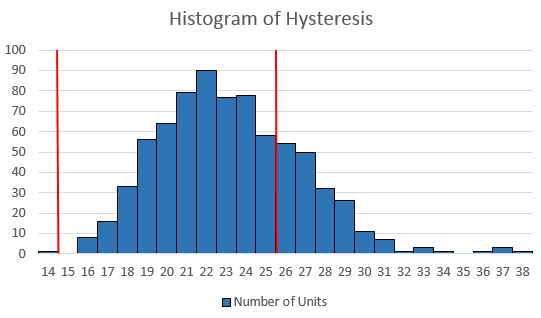
\includegraphics[scale=1]{6hist.png}
\end{center}
Because we know that the ideal operating hysteresis falls between 15 and 25 ft-lbs. As such, we have marked on the graph where these boundaries fall for analysis. We see that a good portion of the data falls within the boundaries, with only one case being below the minimum threshold. The data also appears roughly normal, if skewed to the right. Based on my understanding of the problem, if a part has a higher value of hysteresis this is not necessarily a bad thing, so the rightward skew is not an issue to be corrected. If, however, I am incorrect in that understanding, and the upper bound of 25ft-lbs is a hard cap on the process, then we would seek to reduce the mean torque absorption to place more of the data within the mean. Based on its roughly normal distribution, we seek  to have the mean centered at 20, and most likely three standard deviations of the data to be within the thresholds. This deviation limit will be dependent on company practices.
\end{enumerate}
\end{document}
